\section{Программная реализация инструментария \textit{Adaptor}}
\subsection{Общая информация}
В качестве основного языка реализации системы был выбран \textit{Python}~\cite{python}.

Для реализации статистической обработки данных используется система \textit{Orange}~\cite{orange} и для визуализации графиков "--- модуль \textit{matplotlib}~\cite{matplotlib}.

Инструментарий выполняет эксперименты по запуску программ, исходный код которых доступен экспериментатору. Экспериментатору должна быть доступна большая база исходных кодов для обеспечения возможности производить эксперименты над разнообразными программами, среди которых должны быть и похожие между собой. Последнее требование нужно ввиду необходимости обнаруживать похожесть программ в их поведении при изменении аппаратного обеспечения и настроек сборки.

В качестве репозитория исходных кодов исследуемых программ используется сервер распределённой системы контроля версий \textit{Git}.

В качестве БД для хранения данных о проведённых экспериментах была выбрана \textit{CouchDB}, поскольку она хорошо подходит для сильно распределённых систем (что важно для обеспечения работы отдельных исследователей в различных организациях) и накопления редко меняющихся данных.

Для удобной работы с инструментарием рекомендуется использовать интерпретатор \textit{ipython}~\cite{ipython}. Он предоставляет графическую оболочку языка \textit{Python}, которая позволяет строить графики в том же окне, сохранять сессии использования интерпретатора и имеет хорошую поддержку автодополнения команд и документации.

Инструментарий \textit{Adaptor} имеет базовую поддержку сценариев исследований. Сценарий "--- это набор действий вида <<собрать программу>>, <<запустить программу с измерением времени>>, <<построить график зависимости времени от компилятора>> и т.\,д. Он может задаваться интерактивно или в исходном файле в виде функции языка программирования \textit{Python} с использованием \textit{API} инструментария. Система также предоставляет интерфейс для использования её в качестве модуля языка \textit{Python} сторонними пользователями.


\subsection{Архитектура инструметария \textit{Adaptor}}
Инструментарий \textit{Adaptor} построен на клиент-серверной архитектуре.

Схема инструментария представлена на рисунке~\ref{img:architecture}.

\begin{figure}
	\begin{center}
		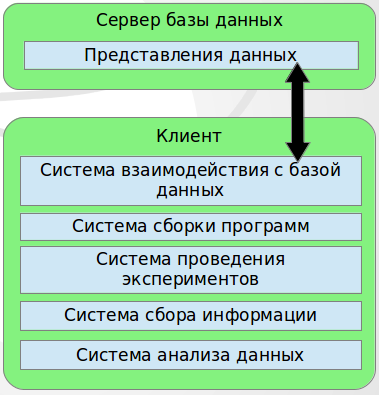
\includegraphics[scale=0.5]{Architecture.png}
	\end{center}
	\label{img:architecture}
	\caption{Архитектура инструментария \textit{Adaptor}}
\end{figure}

\subsection{Структура инструментария}

\paragraph{Компонент сервера}
Компонент представления данных обеспечивает доступ к базе данных.

\paragraph{Компоненты клиента}

\begin{itemize}
	\item Компонент взаимодействия с базой данных. Производит сохранение данных о проведённых экспериментов в локальную или удалённую базу данных.
	\item Компонент сборки программ. Осуществляет сборку исследуемых программ на ЯП \textit{C} в исполняемые файлы.
	\item Компонент проведения экспериментов. Производит запуск исследуемых программ и измерение времени исполнения.
	\item Компонент сбора информации. Осуществляет сбор информации о программно-аппаратной платформе, на которой исполняется исследуемая программа.
	\item Компонент анализа данных. Осуществляет обработку экспериментальных данных с целью выявления зависимости производительности от программно-аппаратных характеристик.
\end{itemize}


\subsection{Эксперимент по оптимизации программы}
Эксперимент состоит в следующем.

\begin{enumerate}
	\item Система собирает программу с определёнными настройками сборки (базовый уровень оптимизации, набор флагов тонких настроек оптимизации и др.).

	\item Система запускает программу в контролируемом окружении с определёнными аргументами и производит измерение полного времени исполнения программы.

	\item Система сохраняет данные о сборке и запуске программы в базу данных для последующего анализа и обработки.
\end{enumerate}

\subsection{Конвейер обработки данных в системе Orange}
\label{orange-pipeline}

На рисунке \ref{img:series30} изображён конвейер статистической обработки данных в системе \textit{Orange}. Здесь он приведён целиком, в уменьшенном виде, для понимания общего расположения компонентов.

Конвейер имеет такой вид для всех трёх серий экспериментов. Далее мы рассмотрим части конвейера по отдельности и опишем каждый компонент, используемый в схеме анализа данных, изображённой на указанном выше рисунке.

\begin{figure}
    \center{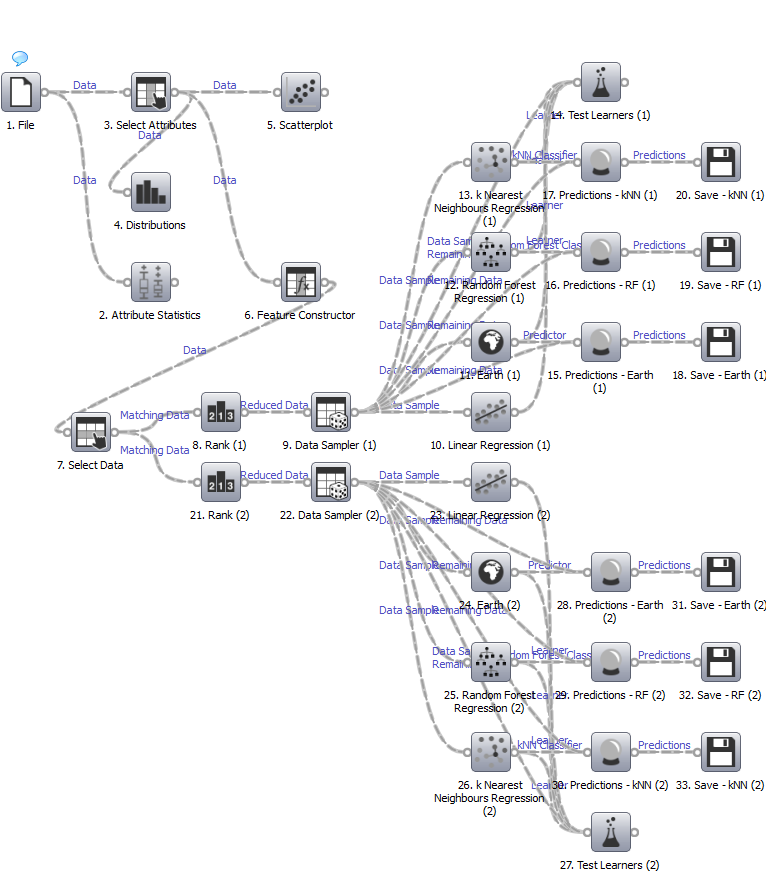
\includegraphics[scale=0.375]{series30}}
    \caption{Конвейер обработки данных в системе \textit{Orange}}
    \label{img:series30}
\end{figure}

Первая часть конвейера "--- предварительная обработка данных перед построением модели. Она изображена на рисунке~\ref{img:series30-1}.

\begin{figure}
    \center{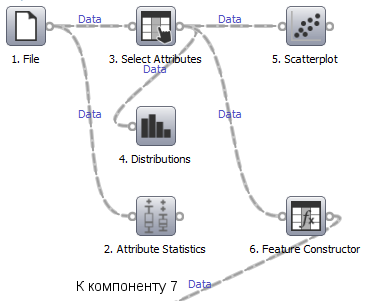
\includegraphics[scale=1]{series30-1}}
    \caption{Конвейер обработки данных в системе \textit{Orange}. Часть 1 "--- предварительная обработка}
    \label{img:series30-1}
\end{figure}

Обработка данных в системе начинается с чтения входных данных в формате \textit{CSV} из файла "--- за это отвечает компонент \texttt{1.\,File}, находящийся в левом верхнем углу схемы.

Входной файл содержит таблицу, в которой столбцы "--- это названия свойств эксперимента, полученных во время его выполнения в инструментарии, а строки "--- собственно значения этих свойств. В таблице содержатся следующие данные: \texttt{id} "--- уникальный идентификатор эксперимента, \texttt{datetime} "--- время его проведения в GMT, \texttt{time} "--- время исполнения программы,  \texttt{program\_name} "--- название программы, \texttt{compiler} "--- название используемого компилятора, \texttt{base\_opt} "--- базовый уровень оптимизации программы компилятором, \texttt{optimization\_flags}  "--- дополнительные настройки оптимизации, \texttt{width} "--- число столбцов в обрабатываемой матрице, \texttt{height} "--- число строк в обрабатываемой матрице, \texttt{cpu\_name} "--- название процессора, на котором исполнялась программа, \texttt{cpu\_mhz} "--- частота процессора, \texttt{cpu\_cache} "--- объём кэша третьего уровня.

Все остальные свойства (например, \texttt{apic} и \texttt{vme}) "--- двоичные свойства наличия у процессора поддержки определённой возможности, такой как, например, набора инструкций \textit{SSE}.

Отметим, что пунктирные линии на схеме обозначают передачу данных из одного компонента обработки данных в другой. Схема представляет собой дерево с корнем в узле \texttt{1.\,File}, причём данные передаются от корня к листьям. Таким образом, из узлов, которые не имеют дочерних, информация дальше не передаётся. Если у узла несколько дочерних узлов, данные передаются от родителя каждому ребёнку данного узла.

Компонент \texttt{2.\,Attribute~Statistics} используется для сбора и показа статистических показателей различных признаков экспериментов, содержащихся в наборе данных -- например, таких, как среднее и медианное значение признака. Выводимые им изображения можно найти в Приложении.

Компонент \texttt{3.\,Select~Attributes} применяется с целью установления структуры набора данных "--- в нём определяется, какие свойства экспериментов являются исходными данными для моделирования (признаками), а какие "--- выходными данными (предсказанными значениями). В данном случае все свойства экспериментов, кроме свойства \texttt{time} (время исполнения программы), являются признаками. Свойство \texttt{time} предсказывается моделью.

Компонент \texttt{4.\,Distributions} отображает распределения различных атрибутов набора данных.

Компонент \texttt{5.\,Scatterplot} строит точечные графики зависимости времени исполнения программы от других свойств эксперимента. Пример такого графика можно найти в Приложении. На нём завершается предварительный анализ входных данных.

Компонент \texttt{6.\,Feature Constructor} используется для создания дополнительного свойства эксперимента из уже присутствующих в наборе данных "--- свойства \texttt{size}, определяемого как $size = height \cdot width$ и имеющего смысл агрегированного размера обрабатываемой программой \texttt{symm} матрицы.

Компонент \texttt{7.\,Select~Data} может использоваться для фильтрации данных по различным признакам. Например, он может быть использован для удаления из набора данных всех экспериментов, для которых измеренное время исполнения оказалось менее 0,001 с вследствие артефактов измерения. Такая фильтрация может увеличить качество предсказания, поскольку результаты, которые очевидно являются шумом, удаляются из набора данных. Однако, в конечных версиях рассмотренных моделей данный компонент не был задействован, поскольку он требует тонкой настройки и снижает степень автоматизации моделирования.

На этом предварительная обработка данных завершается и начинается собственно построение модели. Компоненты под номерами с 8 по 20 и с 20 по 33 полностью аналогичны. Они представляют собой две ветви конвейера, в одной из которых (с компонентами 8--20) используется простейшая модель на основе единственного признака, а в другой (с компонентами 20--33) "--- более сложная модель на основе четырёх или пяти признаков.

Опишем обе ветви конвейера, начиная с части, отвечающей за ранжирование признаков и выборку объектов. Эта часть схемы изображена на рисунке~\ref{img:series30-2}.

\begin{figure}
    \center{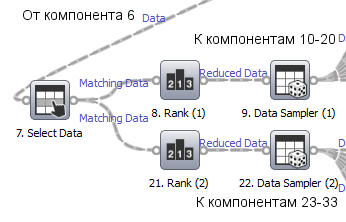
\includegraphics[scale=1]{series30-2}}
    \caption{Конвейер обработки данных в системе \textit{Orange}. Часть 2 "--- ранжирование признаков и выборка объектов}
    \label{img:series30-2}
\end{figure}

Компонент \texttt{8.\,Rank~(1)} и его аналог \texttt{21.\,Rank~(2)}  выбирает $S$ наиболее значимых признаков набора данных, при этом $S = 1$ для компонента 8 и $S = 4$ или $S = 5$ для компонента 21. Выбор $S = 4$ или $S = 5$ зависит от результата работы алгоритма выделения важных признаков и для первой серии экспериментов $S = 4$, а для второй и третьей "--- $S = 5$. Согласно рассуждениям, приведённым ниже в разделе~\ref{choice-of-feature-ranking-algorithm}, в качестве алгоритма ранжирования признаков во всех случаях используется алгоритм \textit{Earth}.

Остановимся подробнее на выборе алгоритма ранжирования признаков.

\paragraph{Алгоритм ранжирования признаков}
\label{choice-of-feature-ranking-algorithm}

В системе статистической обработки данных Orange доступны следующие алгоритмы ранжирования признаков модели: \textit{Relief~F, MSE, Earth Importance} и \textit{Random Forest Importance}. В ходе изучения третьей серии экспериментов были получены результаты ранжирования признаков, показанные на рисунке~\ref{img:ranking-full}.

\begin{figure}
    \center{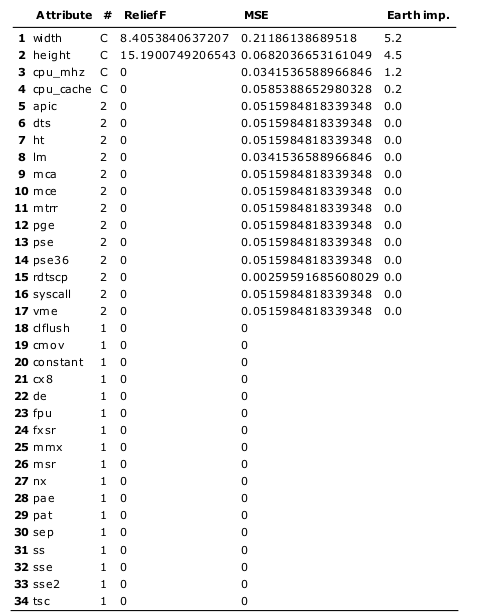
\includegraphics[scale=0.75]{ranking-full}}
    \caption{Сравнение алгоритмов ранжирования признаков модели}
    \label{img:ranking-full}
\end{figure}

Как можно видеть, алгоритм \textit{Relief~F} показал результаты, целиком отбрасывающие влияние свойств \texttt{cpu\_mhz} и \texttt{cpu\_cache}, а также всех остальных особенностей аппаратной платформы. Это заведомо неверно, поскольку известно, что характеристики аппаратного обеспечения влияют на производительность программы. Этот алгоритм выделил только два самых очевидных свойства, оказывающих влияние на производительность.

Алгоритм \textit{MSE} также присвоил наибольшие веса свойствам \texttt{width} и \texttt{height}, а на третье место по важности поставил \texttt{cpu\_cache}, что выглядит разумно. Однако, данный алгоритм присвоил одинаковые веса многим признакам, которые просто коррелируют с изменением свойств \texttt{cpu\_mhz} и \texttt{cpu\_cache}, но не обнаружил корреляции -- таким образом, свойства \texttt{apic, dts} и другие получили вес $0,05159...$. При этом истинно важный признак \texttt{cpu\_mhz} был оценён важностью, меньшей чем у всех этих коррелирующих признаков, что свидетельствует о невозможности применения этого алгоритма для нашей задачи.

Алгоритм \textit{Earth Importance} выявил все четыре признака, которые являются важными в нашей модели -- число строк и столбцов в обрабатываемой матрице, частоту используемого процессора и объём его кэша. При этом <<паразитные>> коррелирующие признаки не были оценены алгоритмом как важные "--- таким образом мы избавляемся от лишних свойств в модели и делаем её минимально необходимой для адекватного описания предметной области.

Алгоритм \textit{Random Forest Importance} отработал на нашем наборе данных некорректно, вызвав программную ошибку в системе Orange. Он был исключён из дальнейшего рассмотрения.

Таким образом, мы выбираем \textit{Earth Importance} в качестве алгоритма ранжирования признаков.

Теперь продолжим рассмотрение конвейера обработки данных в системе \textit{Orange}.

Компоненты \texttt{9.\,Data~Sampler~(1)} и \texttt{22.\,Data~Sampler~(2)} производят случайный отбор 70\% данных из набора в учебный набор, а остальных 30\% "--- в проверочный набор данных. Это необходимо для проведения перекрёстной проверки, которая в данном случае является одно-проходной ввиду ограниченных ресурсов времени и невысокой степени автоматизации осуществления перекрёстной проверки в системе \textit{Orange}. При этом компонент 9 работает с моделью, построенной на основе единственного признака, который был оценён, как наиболее важный, компонентом 8. Компонент 22 работает с моделью на основе четырёх или пяти признаков, наиболее важных по результатам работы компонента 21. Далее мы не будем останавливаться на различиях моделей в ветвях (8--20) и (20--33).

На этом вторая часть схемы заканчивается и мы переходим собственно к обучению предсказателей для двух моделей "--- простейшей (с одним признаком) и более сложной (с четырьмя или пятью признаками).

Две последние части обработки данных в системе \textit{Orange} полностью аналогичны и отличаются тем, что первая (описывающая компоненты~10--20) получает данные от компонента~9, а вторая (компоненты~23--33) "--- от компонента~22. Это данные, включающие в себя один признак эксперимента и несколько (четыре или пять) признаков эксперимента, соответственно.

\begin{figure}
    \center{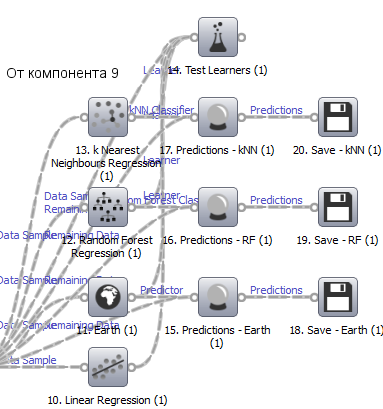
\includegraphics[scale=1]{series30-3}}
    \caption{Конвейер обработки данных в системе \textit{Orange}. Часть 3 "--- построение простейшей модели}
    \label{img:series30-3}
\end{figure}

Компоненты \texttt{10.\,Linear~Regression~(1)} и \texttt{23.\,Linear~Regression~(2)} строят модели линейной регрессии на основе экспериментальных данных. Эти модели являются образцовыми. Это значит, что качество результатов данных моделей является нижней границей для качества результатов любых других моделей. Поскольку линейная регрессия является простейшим предсказателем, рассмотрение моделей, которые дают результаты хуже, чем линейная регрессия, не имеет смысла. Модели из компонентов 10 и 23 передаются в компоненты 14 и 27 соответственно, где те сравниваются с другими предсказателями по нескольким метрикам (см. ниже).

\begin{figure}
    \center{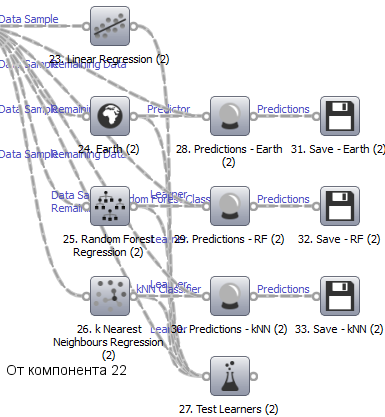
\includegraphics[scale=1]{series30-4}}
    \caption{Конвейер обработки данных в системе \textit{Orange}. Часть 4 "--- построение более сложной модели}
    \label{img:series30-4}
\end{figure}

Компоненты \texttt{11.\,Earth~(1), 12.\,Random~Forest Regression~(1), 13.\,k~Nearest~Neighbours Regression~(1)} и \texttt{24.\,Earth~(2), 25.~Random~Forest Regression~(2), 26.\,k~Nearest~Neighbours Regression~(2)} являются модулями построения предсказателей \textit{Earth, Random~Forest} и \textit{kNN} для ветвей (8--20) и (20--33) соответственно.

После обучения предсказателей их параметры передаются в компоненты сравнения качества результатов \texttt{14.\,Test~Learners~(1)} и \texttt{27.\,Test~Learners~(2)}. Кроме этого, они используются для построения предсказаний в компонентах \texttt{15.\,Predictions - Earth~(1), 16.\,Predictions - RF~(1), 17.\,Predictions - kNN~(1)} и {28.\,Predictions - Earth~(2), 29.\,Predictions - RF~(2), 30.\,Predictions - kNN~(2)} соответсвенно.

После построения предсказаний, они сохраняются в файлах \textit{CSV} с помощью компонентов \texttt{18.\,Save - Earth~(1), 19.\,Save - RF~(1), 20.\,Save - kNN~(1)} и \texttt{31.\,Save - Earth~(2), 32.\,Save - RF~(2), 33.\,Save - kNN~(2)} в формате, аналогичном формату исходного файла, загруженного компонентом \texttt{1.\,File}.